\chapter{Números complejos}\label{numcomp}

Los números complejos son una extensión de los números reales que surgieron de la necesidad de calcular todas las raíces de un polinomio y darle sentido al Teorema Fundamental del Álgebra, el cual establece que todo polinomio de grado $n$ tiene exactamente $n$ raíces contando multiplicidades. Su aplicación es esencial en matemáticas, física e ingeniería. Este capítulo presenta su definición, propiedades básicas y su relación con el Teorema Fundamental del Álgebra.

\section{Propiedades básicas}

\begin{definition}[Número complejo]
Un número complejo es un número de la forma $$z=x+iy$$ donde $x$ y $y$ son números reales e $i$ es la unidad imaginaria definida como $i^2=-1$. El valor $x$ se denomina \textbf{parte real} y el valor $y$ \textbf{parte imaginaria}. El conjunto de todos los números complejos se denota por $\mathbb{C}$.
\end{definition}

\begin{rem} 
En ingeniería, la unidad imaginaria suele representarse como $j$ en lugar de $i$. Esta diferencia es puramente notacional. En este texto se utiliza la convención matemática $i$ para la unidad imaginaria.
\end{rem}

En este capítulo se estudiarán las propiedades básicas de los números complejos y su representación geométrica en el plano complejo. Se inicia con la definición de las operaciones básicas:

\begin{definition}[Operaciones básicas]
Sean $z_1=x_1+iy_1$ y $z_2=x_2+iy_2$ números complejos, se definen:
\begin{itemize}
\item \textbf{Suma:} $z_1+z_2=\left( x_1+x_2 \right) + i\left( y_1+y_2 \right)$.
\item \textbf{Multiplicación:} $z_1z_2=\left(x_1x_2-y_1y_2\right)+i\left(x_1y_2+x_2y_1\right)$.
\item \textbf{Conjugado:} $\overline{z_1}= x_1-iy_1$. En algunos textos avanzados, el conjugado se denota por $z^{*}$. Para evitar confusiones, aquí se usará la notación con línea superpuesta.
\end{itemize} 
\end{definition}

Estas operaciones dotan a los números complejos de la estructura de \textbf{campo}, fundamental para espacios vectoriales (ver Definición \ref{defespvectorial}). La demostración de las siguientes propiedades se propone como ejercicio.

\begin{theorem}[Propiedades de campo de los números complejos]
Sean $z_1,z_2$ y $z_3 \in \mathbb{C}$, entonces:
\begin{enumerate}[$1.$]
\item \textbf{Cerradura bajo la suma y la multiplicación:} $z_1+z_2$ y $z_1z_2$ $\in \mathbb{C}$.
\item \textbf{Asociatividad:} $\left(z_1+z_2 \right)+z_3=z_1+\left( z_2+z_3 \right)$ y $\left( z_1z_2 \right)z_3=z_1\left( z_2z_3 \right)$. 
\item \textbf{Elementos neutros:} Existen $\mathbf{0}=0+0i$ y $1=1+0i \in \mathbb{C}$ tales que $z_1+\mathbf{0}=z_1$ y $1 \cdot z_1=z_1$.
\item \textbf{Inversos:} Existe $-z_1=-x_1-iy_1 \in \mathbb{C}$ tal que $z_1+(-z_1)=\mathbf{0}$. Si $z_1\neq \mathbf{0}$, existe $z_1^{-1}=\dfrac{x_1}{x_1^2+y_1^2}-i\dfrac{y_1}{x_1^2+y_1^2}\in \mathbb{C}$ tal que $z_1z_1^{-1}=1$.
\item \textbf{Distributividad:} $z_1(z_2+z_3)=z_1z_2+z_1z_3$.
\end{enumerate}
\end{theorem}

\begin{prob}  (\cite{andreescu2014complex}, p. 19, Problema 1) Considere los complejos $z_1=1+2i$, $z_2=-2+3i$ y $z_3=1-i$. Calcule:
\begin{multicols}{2}
\begin{enumerate}[$(a)$]
\item $z_1+z_2+z_3$.
\item $z_1z_2z_3$.
\item $\dfrac{z_1^2 + z_2^2}{z_2^2+z_3^2}$.
\item $z_1^2 + z_2^2 +z_3^2$.
\end{enumerate}
\end{multicols}
\begin{myproof}	
$(a)$ Sumando las partes reales e imaginarias:
\begin{equation}
z_1+z_2+z_3 = (1+2i)+(-2+3i)+(1-i)=(1-2+1)+(2+3-1)i= \boxed{0+4i}.
\end{equation}

$(b)$ Calculando paso a paso y utilizando $i^2=-1$:
\begin{align*}
z_1z_2z_3 &= (1+2i)(-2+3i)(1-i)\\
&= (-2+3i+4i+6i^2)(1-i)\\
&= (-2+3i+4i-6)(1-i)\\
&= (-8+7i)(1-i)\\
&= -8+8i+7i^2-7i\\
&= -8+8i-7-7i\\
&= \boxed{-15+i}
\end{align*}

$(c)$ Calculando cada término:
\begin{align*}
z_1^2 &= (1+2i)^2 = 1+4i+4i^2 = 1+4i-4 = -3+4i\\
z_2^2 &= (-2+3i)^2 = 4-12i+9i^2 = 4-12i-9 = -5-12i\\
z_3^2 &= (1-i)^2 = 1-2i+i^2 = 1-2i-1 = -2i
\end{align*}

Por lo tanto:
\begin{align*}
\dfrac{z_1^2 + z_2^2}{z_2^2+z_3^2} &= \dfrac{(-3+4i) + (-5-12i)}{(-5-12i)+(-2i)}\\
&= \dfrac{-8-8i}{-5-14i}\\
\end{align*}

Multiplicando numerador y denominador por el conjugado del denominador:
\begin{align*}
\dfrac{-8-8i}{-5-14i} &= \dfrac{(-8-8i)(-5+14i)}{(-5-14i)(-5+14i)}\\
&= \dfrac{40+112i+40i-112i^2}{25+70i-70i-196i^2}\\
&= \dfrac{40+152i+112}{25+196}\\
&= \dfrac{152+152i}{221}\\
&= \boxed{\frac{152}{221}+\frac{152}{221}i}
\end{align*}

$(d)$ Utilizando los cálculos previos:
\begin{align*}
z_1^2 + z_2^2 +z_3^2 &= (-3+4i) + (-5-12i) + (-2i)\\
&= -8-10i
\end{align*}
\end{myproof}
\end{prob}

\begin{prob} Demuestre que $z$ es real si y solo si es igual a su conjugado.

\begin{myproof}	
Sea $z=a+bi$ un número complejo, donde $a$ y $b$ son números reales. El conjugado de $z$ es $\overline{z}=a-bi$. 

$(\Rightarrow)$ Si $z$ es real, entonces $z=a$ con $b=0$. Por tanto, $\overline{z}=a-0i=a=z$.

$(\Leftarrow)$ Si $z=\overline{z}$, entonces $a+bi=a-bi$. Esto implica que $2bi=0$, lo que solo es posible si $b=0$. Por lo tanto, $z=a$ es un número real.

En conclusión, $z$ es real si y solo si $z=\overline{z}$.
\end{myproof}
\end{prob}


\begin{prob} (\cite{andreescu2014complex}, p. 19, Problema 9) Encuentre los números reales $x,$ $y$ tales que $\dfrac{x-3}{3+i}+\dfrac{y-3}{3-i}=i.$
\begin{myproof}	
Multiplicando ambos lados por el denominador común $(3+i)(3-i)=9+1=10$:
\begin{align*}
\dfrac{x-3}{3+i}+\dfrac{y-3}{3-i}&=i\\
(x-3)(3-i)+(y-3)(3+i)&=10i\\
3x-xi-9+3i+3y+yi-9-3i&=10i\\
(3x+3y-18)+i(-x+y)&=10i
\end{align*}

Igualando partes reales e imaginarias:
\begin{align*}
3x+3y-18&=0\\
-x+y&=10
\end{align*}

De la segunda ecuación: $y=10+x$. Sustituyendo en la primera:
\begin{align*}
3x+3(10+x)-18&=0\\
3x+30+3x-18&=0\\
6x+12&=0\\
6x&=-12\\
x&=-2
\end{align*}

Por lo tanto, $\boxed{x=-2}$ y $\boxed{y=10+(-2)=8}$.
\end{myproof}
\end{prob}

La forma presentada anteriormente se denomina \textbf{forma binomial} o \textbf{cartesiana} de un número complejo. También es posible representar un número complejo como una pareja ordenada $(x,y)$ de números reales, donde la parte real se grafica en el eje $X$ y la parte imaginaria en el eje $Y$. Esta es conocida como la \textbf{representación geométrica} del complejo $z$.

\begin{prob} Calcule la representación geométrica del complejo $z=-5-4i.$ \label{formageometrica54i}
\begin{myproof} 
La parte real del complejo $z$ es $-5$ y la parte imaginaria es $-4$. Por tanto, $z$ corresponde al punto $(-5,-4)$ en el plano complejo. Su representación geométrica es:

\begin{figure}[H]
\centering
\begin{tikzpicture}[line cap=round,line join=round,>=triangle 45,x=0.5cm,y=0.5cm]
\begin{axis}[
x=0.5cm,y=0.5cm,
axis lines=middle,
ymajorgrids=true,
xmajorgrids=true,
xmin=-6.00,
xmax=2.5,
ymin=-4.74,
ymax=1.02,
xtick={-6.0,-5.0,...,1.0},
ytick={-4.0,-3.0,...,1.0},]
\clip(-6.,-4.74) rectangle (1.56,1.02);
 
\draw [fill=red!85!black] (-5.,-4.) circle (2.5pt);
\draw[color=red!85!black] (-4.86,-3.63) node {$z=-5-4i$};
 \draw[color=black] (0.8,-0.5) node {Eje Real};
 \draw[color=black] (-2,0.5) node {Eje Imaginario};
\end{axis}
\end{tikzpicture}
\caption{Representación geométrica del complejo $-5-4i.$}
\end{figure}
\end{myproof}
\end{prob} 

Haciendo uso de las coordenadas polares, podemos obtener otra representación del número complejo $z$:

\begin{definition}[Módulo y argumento]\label{modnumcom}
Sea $z=x+iy$ un número complejo, y $P$ el punto en el plano cartesiano que lo representa. El \textbf{módulo} de $z$, denotado por $\abs{z}$, es la distancia desde el origen $O$ hasta el punto $P$, dado por $\abs{z}=\sqrt{x^2+y^2}$. El \textbf{argumento} de $z$, denotado por $\text{arg}(z)$, es el ángulo medido desde la parte positiva del eje real hasta el segmento $\overline{OP}$. Aunque el argumento puede tomar cualquier valor que difiera en múltiplos de $2\pi$, se suele considerar el \textbf{argumento principal} en el intervalo $[0,2\pi)$.
\end{definition}

Antes de presentar la forma polar, introducimos una de las fórmulas más importantes en matemáticas, cuya demostración se hará en el Teorema \ref{demformeuler}.

\begin{theorem}[Fórmula de Euler]\label{formeuler} Para cualquier número real $\theta$:
$$\mathrm{e}^{i\theta}=\cos \theta + i \sen \theta.$$
\end{theorem}

\begin{definition}[Forma polar] 
Sea $z=x+iy$ un número complejo con módulo $\abs{z}$ y argumento $\theta=\text{arg}(z)$. La forma polar de $z$ se expresa como:
$$z=\abs{z}\mathrm{e}^{i\theta}.$$
\end{definition}

Una ventaja significativa de la forma polar es la simplificación de las operaciones de multiplicación y división:

\begin{theorem}[Multiplicación y división en forma polar]
Sean $z_1=\abs{z_1}\mathrm{e}^{i\theta_1}$ y $z_2=\abs{z_2}\mathrm{e}^{i\theta_2}$ números complejos. Entonces:
\begin{enumerate}[$1.$]
\item $z_1z_2=\abs{z_1}\abs{z_2}\mathrm{e}^{i(\theta_1 + \theta_2)}.$
\item $\dfrac{z_1}{z_2}=\dfrac{\abs{z_1}}{\abs{z_2}}\mathrm{e}^{i(\theta_1 - \theta_2)}.$
\end{enumerate}
\end{theorem}

\begin{rem} 
De este teorema se deduce que multiplicar complejos en forma polar equivale a multiplicar sus módulos y sumar sus argumentos, mientras que dividir complejos equivale a dividir sus módulos y restar sus argumentos. Para estas operaciones es importante considerar el cuadrante y posiblemente ajustar para obtener el argumento principal.
\end{rem}

\begin{prob} Encuentre la forma polar del número complejo $z=-5-4i.$ ¿Cuál es el efecto geométrico en el plano complejo de multiplicar y dividir por este número? Justifique su respuesta. \label{formapolar54i}

\begin{myproof}
Para encontrar la forma polar de $z=-5-4i$, calculamos:

El módulo: $|z|=\sqrt{(-5)^2+(-4)^2}=\sqrt{25+16}=\sqrt{41}$.

Para el argumento, calculamos $\tan\theta = \frac{-4}{-5}=\frac{4}{5}$, lo que da $\theta = \arctan\left(\frac{4}{5}\right) \approx 0.6747$ radianes. Como $z$ se encuentra en el tercer cuadrante (tanto $x$ como $y$ son negativos), debemos sumar $\pi$ al valor obtenido:
$$\text{arg}(z) = \pi+\arctan\left(\frac{4}{5}\right) \approx 3.8163 \text{ radianes}.$$

Por tanto, la forma polar de $z$ es $\boxed{z=\sqrt{41}\,\mathrm{e}^{i\cdot 3.8163}}$.

Respecto al efecto geométrico:
- Multiplicar un número complejo por $z$ tiene dos efectos: (1) una dilatación por un factor de $\sqrt{41} \approx 6.40$ y (2) una rotación en sentido antihorario de aproximadamente $3.8163$ radianes (218.8°).
- Dividir por $z$ produce: (1) una contracción por un factor de $\frac{1}{\sqrt{41}} \approx 0.156$ y (2) una rotación en sentido horario de $3.8163$ radianes.
\end{myproof}
\end{prob}

Es posible verificar los resultados de los problemas \ref{formageometrica54i} y \ref{formapolar54i} mediante el siguiente programa en \texttt{Python 3.x}:

\begin{prob} Use el lenguaje de programación \texttt{Python 3.x} para calcular la forma geométrica y polar del número complejo $-5-4i$.
\begin{myproof}
\begin{lstlisting}[label={lst:complejo},basicstyle=\footnotesize]
import cmath
import matplotlib.pyplot as plt

def calcular_modulo_argumento(numero_complejo):
    modulo = abs(numero_complejo)
    argumento = cmath.phase(numero_complejo)
    
    # Normalizar el argumento al intervalo [0, 2π)
    if argumento < 0:
        argumento += 2 * cmath.pi
    elif argumento > 2 * cmath.pi:
        argumento %= 2 * cmath.pi
    
    return modulo, argumento

# Entrada de valores
real_part = float(input("Parte real: "))
imag_part = float(input("Parte imaginaria, sin la i: "))
numero_complejo = complex(real_part, imag_part)

# Cálculo de módulo y argumento
modulo, argumento = calcular_modulo_argumento(numero_complejo)
print(f'Módulo: {modulo}')
print(f'Argumento: {argumento} radianes')

# Visualización gráfica
plt.figure(figsize=(8, 8))
plt.scatter(real_part, imag_part, color='red', marker='x', label='Número complejo')
plt.xlabel('Parte Real')
plt.ylabel('Parte Imaginaria')
plt.title('Representación en el Plano Complejo')
plt.axhline(0, color='black', linewidth=0.5)
plt.axvline(0, color='black', linewidth=0.5)
plt.grid(color='gray', linestyle='--', linewidth=0.5)
plt.legend()
plt.show()
\end{lstlisting}

Este programa genera la siguiente salida:

Parte real: -5

Parte imaginaria, sin la i: -4

Módulo: $6.4031242374328485$

Argumento: $3.8163335958133455$ radianes.

\begin{figure}[H]
\centering
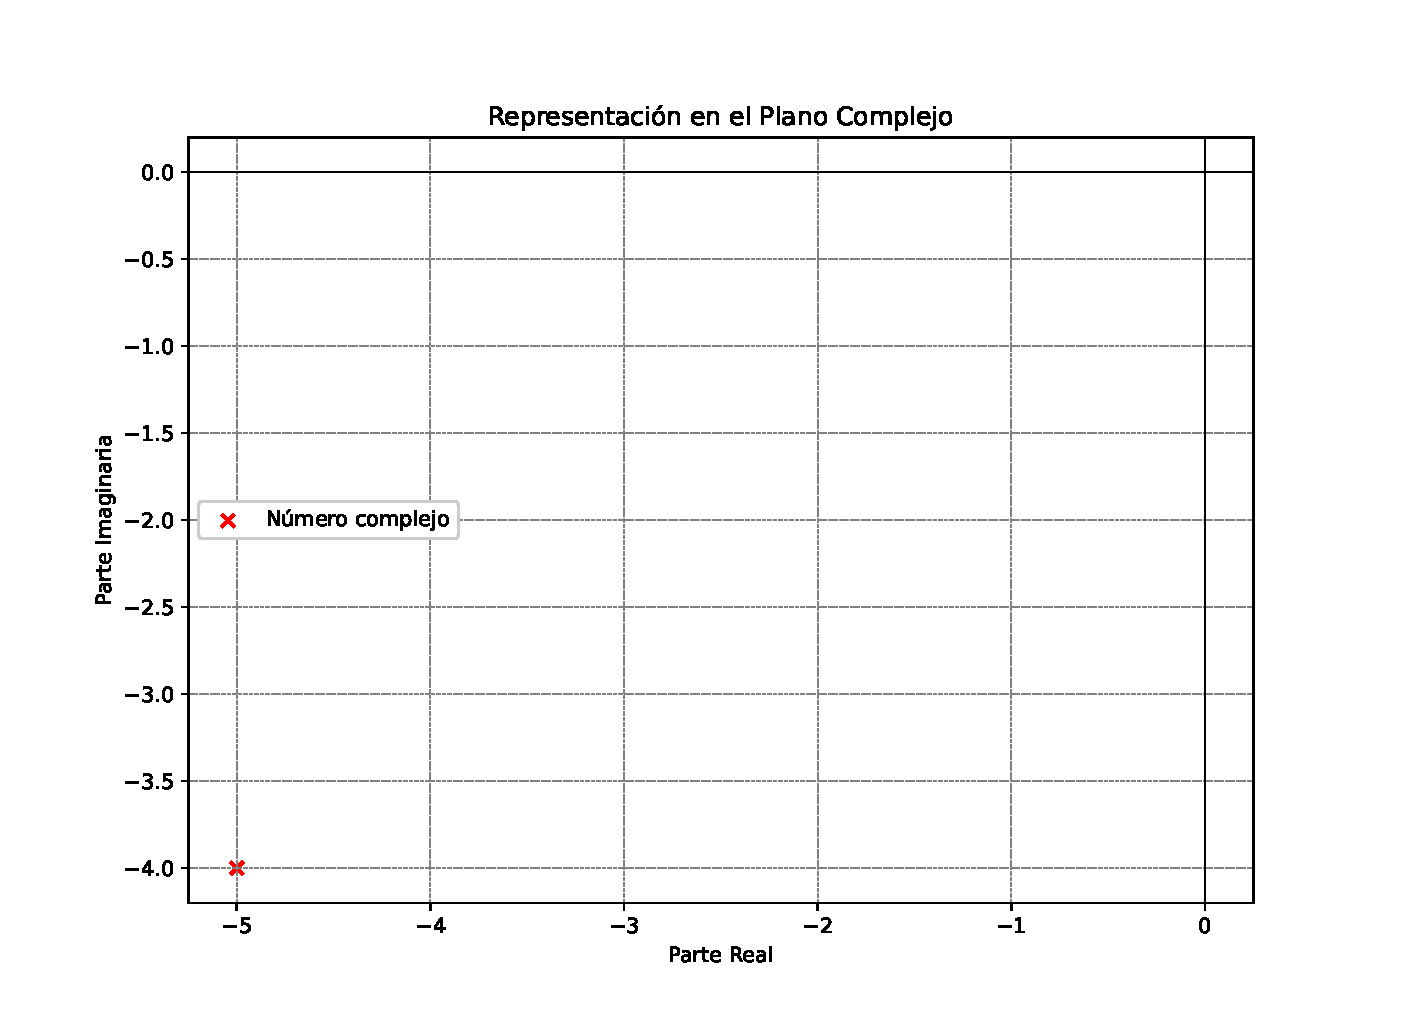
\includegraphics[scale=0.35]{representacioncomplejo.eps}
\caption{Representación gráfica en \texttt{matplotlib} del complejo $-5-4i.$}
\end{figure}

Estos resultados confirman los cálculos realizados en los problemas \ref{formageometrica54i} y \ref{formapolar54i}.
\end{myproof}
\end{prob}

\begin{prob} Sea $z$ un número complejo. Es posible probarse que si $\abs{z}=1,$ con $z\neq 1$ entonces $z=\dfrac{1+it}{1-it},$ con $t\in \mathbb{R}.$  Para el complejo $z=\dfrac{1}{2}+\dfrac{\sqrt{3}}{2}i$ se tiene que  $it$ es igual a %real
				\begin{multicols}{4}
					\begin{enumerate}[$(a)$]
						\item $ \dfrac{ 1-\sqrt{3}}{-3-\sqrt{3}}.$  
						\item $ \dfrac{-1+\sqrt{3}i}{1-\sqrt{3}i}.$  
						\item $ \dfrac{-1+\sqrt{3}}{3+\sqrt{3}}.$  %ok
						\item Ninguna.
					\end{enumerate}
				\end{multicols}							
\begin{myproof}
Observe que si $z=\dfrac{1+it}{1-it},$ entonces 
\begin{align*}
z\left( 1-it \right)&=1+it\\
z-zit&=1+it\\
z-1&=zit+it\\
\dfrac{z-1}{z+1}&=it.
\end{align*}

De esta manera, \begin{align*} it&=\dfrac{\dfrac{1}{2}+\dfrac{\sqrt{3}}{2}i-1}{\dfrac{1}{2}+\dfrac{\sqrt{3}}{2}i+1}=\dfrac{\dfrac{1}{2}+\dfrac{\sqrt{3}}{2}i-1}{\dfrac{1}{2}+\dfrac{\sqrt{3}}{2}i+1}\\
&=\dfrac{1+\sqrt{3}i-2}{1+\sqrt{3}i+2}=\boxed{\dfrac{-1+\sqrt{3}i}{3+\sqrt{3}i}}.
\end{align*}
Por lo cual, la opción correcta es \textbf{Ninguna.}
\end{myproof}
\end{prob}

\begin{prob}  (\cite{andreescu2014complex}, p. 30, Problema 5)
Sean $z_1 = 1+i$ y $z_2 = -1-i$. Encuentre el número complejo $z_3$ tal que el triángulo $z_1$, $z_2$ y $z_3$ sea equilátero.
\end{prob}

\begin{myproof}
El problema tiene dos soluciones, dependiendo del argumento a tomar. Se muestran ambas.

\begin{figure}[H]
\centering
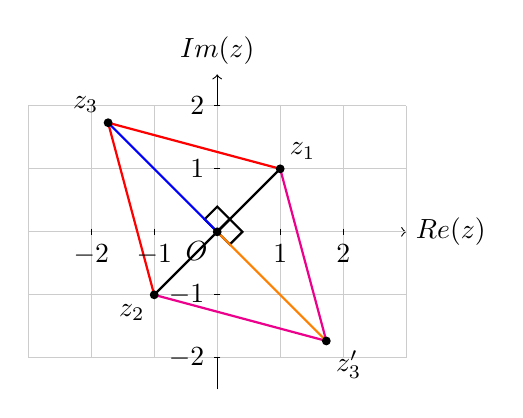
\begin{tikzpicture}[scale=0.8]
% Ejes
\draw[->] (-3,0) -- (3,0) node[right] {$\text{Re}(z)$};
\draw[->] (0,-2.5) -- (0,2.5) node[above] {$\text{Im}(z)$};

% Grilla
\draw[thin,gray!40] (-3,-2) grid (3,2);

% Marcadores de ángulo recto en el origen
\draw[thick] (0.2,0.2) -- (0,0.4) -- (-0.2,0.2) -- (0,0) -- cycle; 
\draw[thick] (0.2,-0.2) -- (0.4,0) -- (0.2,0.2) -- (0,0) -- cycle; 

% Lado principal z1-z2
\draw[thick] (-1,-1) -- (1,1);

% Primer triángulo equilátero
\draw[thick, red] (1,1) -- (-1.732,1.732);
\draw[thick, red] (-1.732,1.732) -- (-1,-1);

% Segundo triángulo equilátero
\draw[thick, magenta] (1,1) -- (1.732,-1.732);
\draw[thick, magenta] (1.732,-1.732) -- (-1,-1);

% Líneas desde el origen (alturas)
\draw[thick, blue] (-1.732,1.732) -- (0,0);
\draw[thick, orange] (1.732,-1.732) -- (0,0);

% Puntos
\fill[black] (1,1) circle (2pt);
\fill[black] (-1,-1) circle (2pt);
\fill[black] (-1.732,1.732) circle (2pt);
\fill[black] (0,0) circle (2pt);
\fill[black] (1.732,-1.732) circle (2pt);

% Etiquetas
\node[above right] at (1,1) {$z_1$};
\node[below left] at (-1,-1) {$z_2$};
\node[above left] at (-1.732,1.732) {$z_3$};
\node[below right] at (1.732,-1.732) {$z_3'$};
\node[below left] at (0,0) {$O$};

% Marcas en los ejes
\foreach \x in {-2,-1,1,2}
    \draw (\x,0.05) -- (\x,-0.05) node[below] {$\x$};
\foreach \y in {-2,-1,1,2}
    \draw (0.05,\y) -- (-0.05,\y) node[left] {$\y$};
\end{tikzpicture}
\caption{Representación gráfica de la solución}
\end{figure}



Observe que si $z_1 = 1+i$ y $z_2 = -1-i$ son vértices, entonces el segmento $\overline{z_1z_2}$ es un lado del triángulo. Como este es equilátero, su altura pasa por el punto medio del segmento, que es precisamente $0+0i$. 

La estrategia es calcular el módulo y argumento del complejo $z_3$ usando propiedades geométricas del triángulo equilátero.



\textbf{Cálculo del argumento:}

El argumento de $z_1$ es $\arg(z_1) = \arctan(1) = \frac{\pi}{4}$. 

Como la altura del triángulo equilátero es perpendicular al lado $\overline{z_1z_2}$, los posibles argumentos de $z_3$ son:
\begin{align}
\arg(z_3) &= \frac{\pi}{4} + \frac{\pi}{2} = \frac{3\pi}{4}\\
\arg(z_3') &= \frac{\pi}{4} - \frac{\pi}{2} = -\frac{\pi}{4} = \frac{7\pi}{4}
\end{align}

\textbf{Cálculo del módulo:}

La longitud del lado del triángulo es:
$$|z_1 - z_2| = |2 + 2i| = 2\sqrt{2}$$

En un triángulo equilátero, si el lado mide $a$, entonces la altura mide $\frac{\sqrt{3}}{2}a$. Por tanto:
$$|z_3| = \frac{\sqrt{3}}{2} \cdot 2\sqrt{2} = \sqrt{6}$$

\textbf{Soluciones finales:}

$$\boxed{z_3 = \sqrt{6} \cdot e^{i\frac{3\pi}{4}} = -\sqrt{3} + i\sqrt{3}}$$

$$\boxed{z_3' = \sqrt{6} \cdot e^{i\frac{7\pi}{4}} = \sqrt{3} - i\sqrt{3}}$$

\end{myproof}

De la multiplicación de números complejos en forma polar se derivan las siguientes propiedades importantes:

\begin{theorem}[Potencias y raíces enésimas de un número complejo] Sea $z=\abs{z}\mathrm{e}^{i\theta}$ un número complejo y $n$ un entero positivo, entonces:
\begin{enumerate}[$1.$]
\item $z^{n}=\abs{z}^n\mathrm{e}^{in\theta}$.
\item \textbf{Fórmula de De Moivre:} $\sqrt[n]{z}=\sqrt[n]{\abs{z}}\cdot \mathrm{e}^{i\frac{\theta+2k\pi}{n}}$ donde $k=0,1,\dots , n-1$.
\end{enumerate}
\end{theorem}

\begin{prob} Determine el valor de verdad de las siguientes afirmaciones donde $z$ y $w\ \in \mathbb{C}$. Si son verdaderas, demuéstrelas; de lo contrario, presente un contraejemplo.

\begin{multicols}{2}
\begin{enumerate}[$a)$]
       \item $z\overline{z}=|z|^2$.
      \item  $|z^n|=|z|^n$.
      \item  Si $\text{Re}(w)\neq 0$, $\text{arg}\left(\dfrac{z}{w}\right)=\dfrac{\text{arg}(z)}{\text{arg}(w)}$.
      \item  Si $z\in\mathbb{R}$, entonces $\text{arg}(z)=\pi$.
\end{enumerate}
\end{multicols}

\begin{myproof}	
\begin{enumerate}[$a)$]
\item Verdadero. \textbf{Demostración:}
Sea $z=a+bi$, entonces $\overline{z}=a-bi$. Por lo tanto:
$$z\overline{z}= (a+bi)(a-bi)= a^2 + abi - abi - b^2i^2 = a^2 + b^2 = |z|^2.$$

\item Verdadero. \textbf{Demostración:} 
Primero demostraremos que para cualesquiera números complejos $w$ y $z$, se cumple que $|wz|=|w||z|$.

Sean $w=a+ib$ y $z=c+di$. Entonces:
\begin{align*}
wz &= (a+ib)(c+di) = (ac-bd) + i(ad+bc)\\
|wz|^2 &= (ac-bd)^2 + (ad+bc)^2\\
&= a^2c^2 - 2abcd + b^2d^2 + a^2d^2 + 2abcd + b^2c^2\\
&= a^2(c^2+d^2) + b^2(c^2+d^2)\\
&= (a^2+b^2)(c^2+d^2)\\
&= |w|^2|z|^2
\end{align*}

Por lo tanto, $|wz| = |w||z|$.

Para demostrar que $|z^n|=|z|^n$ para todo entero positivo $n$, usamos inducción matemática:
- Base ($n=1$): Trivialmente, $|z^1|=|z|^1=|z|$.
- Paso inductivo: Supongamos que $|z^k|=|z|^k$ para algún $k \geq 1$.
- Para $n=k+1$: $|z^{k+1}| = |z^k \cdot z| = |z^k| \cdot |z| = |z|^k \cdot |z| = |z|^{k+1}$

Por el principio de inducción matemática, $|z^n|=|z|^n$ para todo entero positivo $n$.

\item Falso. \textbf{Contraejemplo:} 
Sea $z=1$ y $w=1+i$. 

Calculamos $\dfrac{z}{w} = \dfrac{1}{1+i} = \dfrac{1(1-i)}{(1+i)(1-i)} = \dfrac{1-i}{2}$.

Por lo tanto:
$$\text{arg}\left(\dfrac{z}{w}\right) = \text{arg}\left(\dfrac{1-i}{2}\right) = \text{arg}(1-i) = -\frac{\pi}{4} = \frac{7\pi}{4}$$

Mientras que:
$$\dfrac{\text{arg}(z)}{\text{arg}(w)} = \dfrac{\text{arg}(1)}{\text{arg}(1+i)} = \dfrac{0}{\frac{\pi}{4}} = 0$$

Como $\frac{7\pi}{4} \neq 0$, la afirmación es falsa.

\item Falso. \textbf{Contraejemplo:} 
Sea $z=1 \in \mathbb{R}$. Entonces $\text{arg}(z) = 0 \neq \pi$. 

En realidad, para cualquier número real positivo $z > 0$, tenemos $\text{arg}(z) = 0$, y para cualquier número real negativo $z < 0$, tenemos $\text{arg}(z) = \pi$. La afirmación solo es cierta para números reales negativos.
\end{enumerate}
\end{myproof}
\end{prob}

\begin{prob}  (\cite{andreescu2014complex}, p. 55, Problemas 1 y 3) Use la fórmula de De Moivre para encontrar las raíces cuartas de los siguientes complejos:
\begin{multicols}{2}
\begin{enumerate}[$a)$]
\item $z=-27$.
\item $z=-7+24i$.
\end{enumerate}
\end{multicols}
\begin{myproof}
Para calcular las raíces cuartas de los números complejos dados, primero los expresaremos en forma polar y luego aplicaremos la fórmula de De Moivre.

\begin{enumerate}[$a)$]
\item Para $z=-27$:
   
   El módulo es $|-27| = 27$ y su argumento es $\text{arg}(-27) = \pi$, por lo cual, $z = 27\cdot e^{i\pi}$.
   
   Las raíces cuartas están dadas por:
   $$\sqrt[4]{z} = \sqrt[4]{27}\cdot \mathrm{e}^{i\frac{\pi+2k\pi}{4}}$$
   donde $k=0,1,2,3$.
   
   Dado que $\sqrt[4]{27} \approx 2.28$, tenemos:
   $$\begin{matrix}
   k=0: & \sqrt[4]{27}\cdot\mathrm{e}^{i\frac{\pi}{4}} &\approx& 2.28\cdot\mathrm{e}^{i\frac{\pi}{4}} &\approx& 1.61+1.61i \\
   k=1: & \sqrt[4]{27}\cdot\mathrm{e}^{i\frac{3\pi}{4}} &\approx& 2.28\cdot\mathrm{e}^{i\frac{3\pi}{4}} &\approx& -1.61+1.61i \\
   k=2: & \sqrt[4]{27}\cdot\mathrm{e}^{i\frac{5\pi}{4}} &\approx& 2.28\cdot\mathrm{e}^{i\frac{5\pi}{4}} &\approx& -1.61-1.61i \\
   k=3: & \sqrt[4]{27}\cdot\mathrm{e}^{i\frac{7\pi}{4}} &\approx& 2.28\cdot\mathrm{e}^{i\frac{7\pi}{4}} &\approx& 1.61-1.61i
   \end{matrix}$$

\item Para $z=-7+24i$:
   
   El módulo es $|z| = \sqrt{(-7)^2+(24)^2} = \sqrt{49+576} = \sqrt{625} = 25$.
   
   Para el argumento, como $z$ está en el segundo cuadrante (parte real negativa, parte imaginaria positiva):
   $$\text{arg}(z) = \arctan\left(\frac{24}{-7}\right) + \pi = \arctan(-\frac{24}{7}) + \pi \approx -1.2863 + \pi \approx 1.8553 \text{ radianes}$$
   
   Por lo tanto, $z = 25\cdot e^{i\cdot 1.8553}$.
   
   Las raíces cuartas están dadas por:
   $$\sqrt[4]{z} = \sqrt[4]{25}\cdot \mathrm{e}^{i\frac{1.8553+2k\pi}{4}}$$
   donde $k=0,1,2,3$ y $\sqrt[4]{25} = 2.24$
   
   $$\begin{matrix}
   k=0: & 2.24\cdot\mathrm{e}^{i\frac{1.8553}{4}} &\approx& 2.24\cdot\mathrm{e}^{i\cdot 0.4638} &\approx& 2.02+0.94i \\
   k=1: & 2.24\cdot\mathrm{e}^{i\frac{1.8553+2\pi}{4}} &\approx& 2.24\cdot\mathrm{e}^{i\cdot 2.0344} &\approx& -0.68+2.14i \\
   k=2: & 2.24\cdot\mathrm{e}^{i\frac{1.8553+4\pi}{4}} &\approx& 2.24\cdot\mathrm{e}^{i\cdot 3.6050} &\approx& -2.02-0.94i \\
   k=3: & 2.24\cdot\mathrm{e}^{i\frac{1.8553+6\pi}{4}} &\approx& 2.24\cdot\mathrm{e}^{i\cdot 5.1756} &\approx& 0.68-2.14i
   \end{matrix}$$
\end{enumerate}
\end{myproof}
\end{prob}

\section{Teorema Fundamental del Álgebra}

\begin{definition}[Raíz de un polinomio] 
Sea $p(z)$ un polinomio con coeficientes complejos. Diremos que $\alpha \in \mathbb{C}$ es una raíz de $p(z)$ si $p(\alpha)=0$. Es decir, $\alpha$ es una solución de la ecuación polinómica $p(z)=0$.
\end{definition}

El cálculo de las raíces de un polinomio puede ser un problema muy difícil y se estudia ampliamente en matemáticas, en una rama llamada análisis numérico. Debido a los alcances de este curso, se tratarán polinomios especiales con coeficientes complejos (que incluyen los de coeficientes reales como caso particular) para los cuales sea fácil calcular su factorización. Sin embargo, el siguiente teorema no distingue el tipo de polinomio a estudiar. Este teorema es un resultado muy importante demostrado, entre otros, por \textbf{Carl Friedrich Gauss} (1777--1855), un célebre matemático alemán que nombraremos bastante en este curso.

\begin{theorem}[Teorema Fundamental del Álgebra]\label{tfam}
Todo polinomio no constante $p(z)$ de grado $n \geq 1$ con coeficientes complejos tiene exactamente $n$ raíces en $\mathbb{C}$, contando sus multiplicidades algebraicas.
\end{theorem}

\begin{rem}
La multiplicidad algebraica de una raíz $\alpha$ de un polinomio $p(z)$ es el mayor entero positivo $m$ tal que $(z-\alpha)^m$ divide a $p(z)$. En otras palabras, es el exponente más alto de $(z-\alpha)$ en la factorización completa de $p(z)$. Por ejemplo, si $p(z) = (z-1)^2(z-2)$, entonces $z=1$ es una raíz con multiplicidad algebraica $2$, mientras que $z=2$ es una raíz con multiplicidad algebraica $1$ (o raíz simple). En adelante, cuando se haga referencia a la multiplicidad de una raíz, se entenderá la multiplicidad algebraica ya que luego en la Definición \ref{multiplicidadgeometrica} exténderemos este concepto.
\end{rem}

\begin{prob}(\cite{andreescu2014complex}, p. 55, Problema 7) Use la fórmula de De Moivre para encontrar todas las raíces complejas de los siguientes polinomios:

\begin{multicols}{2}
\begin{enumerate}[$a)$]
\item $z^4-z^2+1=0$
\item $z^7-2iz^4-iz^3-2=0$
\end{enumerate}
\end{multicols}

\begin{myproof}
\begin{enumerate}[$a)$]
\item Tome $w=z^2$ entonces la ecuación se reduce a $w^2-w+1=0$. Usando la fórmula cuadrática las soluciones son  $$w = \frac{-(-1)\pm\sqrt{(-1)^2-4(1)(1)}}{2(1)} = \frac{1\pm\sqrt{-3}}{2} = \frac{1\pm i\sqrt{3}}{2}$$

Note que las soluciones son números complejos, además que $w$ es raíz cuadrada de $z$, por lo cual se calcula la forma polar de cada complejo y sus raíces cuadradas:

\begin{itemize}
\item Para $w=\frac{1+\sqrt{3}i}{2}$:  

$|w| = \sqrt{\left( \frac{1}{2} \right)^2 + \left( \frac{\sqrt{3}}{2} \right)^2} = \sqrt{\frac{1}{4}+\frac{3}{4}} = 1,$ y $\arg(w) = \arctan\left( \frac{\sqrt{3}/2}{1/2} \right) = \arctan(\sqrt{3}) = \frac{\pi}{3}.$


Las raíces cuadradas son $\sqrt{1} e^{i\frac{\frac{\pi}{3}+2k\pi}{2}}$ donde $k=0,1$.

$k=0:   e^{i\frac{\pi/3}{2}} = \boxed{e^{i\frac{\pi}{6}}}$ y $k=1: e^{i\frac{\pi/3+2\pi}{2}} = \boxed{e^{i\frac{7\pi}{6}}}$

\item Para $w=\frac{1-i\sqrt{3}}{2}$:

$|w| = \sqrt{\left( \frac{1}{2} \right)^2 + \left( \frac{\sqrt{3}}{2} \right)^2} = 1$ y $\arg(w) = \arctan\left( \frac{-\sqrt{3}/2}{1/2} \right) = \arctan(-\sqrt{3}) = -\frac{\pi}{3}$


Tomando el argumento principal: $\arg(w) = 2\pi - \frac{\pi}{3} = \frac{5\pi}{3}$.

Las raíces cuadradas son $\sqrt{1} e^{i\frac{\frac{5\pi}{3}+2k\pi}{2}}$ donde $k=0,1$.

$k=0:  e^{i\frac{5\pi/3}{2}} = \boxed{e^{i\frac{5\pi}{6}}}$ y  $k=1: e^{i\frac{5\pi/3+2\pi}{2}} = \boxed{e^{i\frac{11\pi}{6}}}$
\end{itemize}

Finalmente las soluciones de la ecuación son:
$$z_1 = e^{i\frac{\pi}{6}}, \quad z_2 = e^{i\frac{5\pi}{6}}, \quad z_3 = e^{i\frac{7\pi}{6}}, \quad z_4 = e^{i\frac{11\pi}{6}}$$

\item Factorizando la ecuación: $z^7-2iz^4-iz^3-2=z^4(z^3-2i)-i(z^3-2i)=(z^4-i)(z^3-2i)= 0.$

Como los complejos forman un dominio entero, la ecuación se puede resolver calculando los valores de $z$ tales que $z^4=i$ y $z^3=2i$.

\begin{itemize}
\item Para $z^4=i$: $|i|=1$ y $\arg(i)=\frac{\pi}{2}$.

Las raíces cuartas son $e^{i\frac{\frac{\pi}{2}+2k\pi}{4}}$ donde $k=0,1,2,3$.

$k=0:\boxed{e^{i\frac{\pi}{8}}},$ $k=1: \boxed{e^{i\frac{5\pi}{8}}},$ $k=2: \boxed{e^{i\frac{9\pi}{8}}},$ $k=3: \boxed{e^{i\frac{13\pi}{8}}}.$

\item Para $z^3=2i$: $|2i|=2$ y $\arg(2i)=\frac{\pi}{2}$.

Las raíces cúbicas son $\sqrt[3]{2} e^{i\frac{\frac{\pi}{2}+2k\pi}{3}}$ donde $k=0,1,2$.

$k=0: \boxed{\sqrt[3]{2}e^{i\frac{\pi}{6}}},$ $k=1: \boxed{\sqrt[3]{2}e^{i\frac{5\pi}{6}}},$ $k=2: \boxed{\sqrt[3]{2}e^{i\frac{3\pi}{2}}}.$
\end{itemize}

Finalmente las soluciones de la ecuación son:
$z_1 = e^{i\frac{\pi}{8}},$ $z_2 = e^{i\frac{5\pi}{8}},$ $z_3 = e^{i\frac{9\pi}{8}},$ $z_4 = e^{i\frac{13\pi}{8}},$ $z_5 = \sqrt[3]{2}e^{i\frac{\pi}{6}},$ $z_6 = \sqrt[3]{2}e^{i\frac{5\pi}{6}},$ $z_7 = \sqrt[3]{2}e^{i\frac{3\pi}{2}}.$
\end{enumerate}
\end{myproof}
\end{prob}



\section{Problemas propuestos para el capítulo}

\begin{prob} Determine cuál opción es correcta y justifique por qué las demás son incorrectas:

El efecto geométrico de multiplicar por el complejo $w=6\left(\dfrac{3+3i}{3-3i}\right)$ en el plano complejo es:

\begin{enumerate}[$(a)$]
\item sextuplicar el módulo y girar $\dfrac{\pi}{2}$ en sentido horario.
\item duplicar el módulo y girar $\pi$ en sentido antihorario.
\item multiplicar el módulo por $3$ y girar $\dfrac{\pi}{4}$ en sentido horario.
\item multiplicar el módulo por $6$ y girar $\pi$ en sentido antihorario.
\item Ninguna.					
\end{enumerate}


\begin{myproof}
Primero, simplificamos el número complejo dado:
$$
w = 6\left(\frac{3+3i}{3-3i}\right)
$$
Multiplicamos numerador y denominador por el conjugado del denominador:
$$
\frac{3+3i}{3-3i} = \frac{(3+3i)(3+3i)}{(3-3i)(3+3i)} = \frac{(3+3i)^2}{3^2 - (3i)^2}
$$
Calculamos:
$$
(3+3i)^2 = 9 + 18i + 9i^2 = 9 + 18i - 9 = 18i
$$
$$
3^2 - (3i)^2 = 9 - 9i^2 = 9 - (-9) = 18
$$
Entonces:
$$
\frac{3+3i}{3-3i} = \frac{18i}{18} = i
$$
Por lo tanto:
$$
w = 6i
$$

El efecto geométrico de multiplicar por $w=6i$ en el plano complejo es:  multiplicar el módulo por $6$ y girar el ángulo por el argumento de $i$, que es $\frac{\pi}{2}$ en sentido antihorario (positivo).

Ahora analizamos las opciones:

\begin{enumerate}[(a)]
\item \textbf{Sextuplicar el módulo y girar $\frac{\pi}{2}$ en sentido horario.}  
Incorrecta. El giro es en sentido antihorario, no horario.

\item \textbf{Duplicar el módulo y girar $\pi$ en sentido antihorario.}  
Incorrecta. El módulo se multiplica por $6$, no por $2$, y el giro no es $\pi$.

\item \textbf{Multiplicar el módulo por $3$ y girar $\frac{\pi}{4}$ en sentido horario.}  
Incorrecta. El módulo se multiplica por $6$, no por $3$, y el ángulo es $\frac{\pi}{2}$, no $\frac{\pi}{4}$.

\item \textbf{Multiplicar el módulo por $6$ y girar $\pi$ en sentido antihorario.}  
Incorrecta. El giro es de $\frac{\pi}{2}$, no de $\pi$.

\item \textbf{Ninguna.}  
Correcta. Ninguna de las opciones anteriores describe correctamente el efecto de multiplicar por $w=6i$.
\end{enumerate}

Por lo tanto, la opción correcta es la \textbf{(e) Ninguna}.
\end{myproof}

\end{prob}



\begin{prob}\label{compsombreado}
Determine cuál de las siguientes opciones representa el subconjunto de los números complejos sombreado en la gráfica:


\begin{figure}[H]
\centering 		
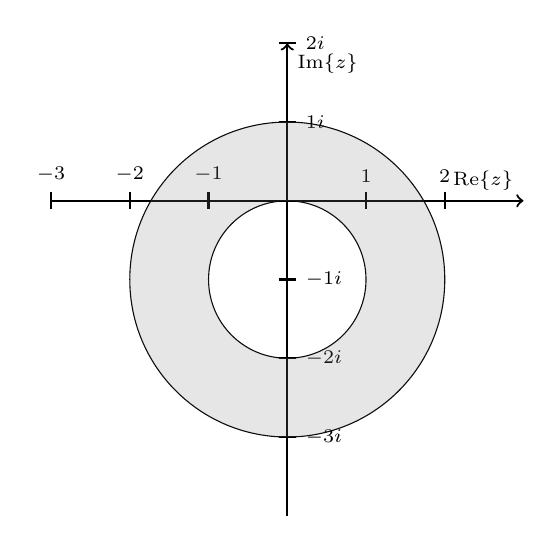
\begin{tikzpicture}
\begin{scope}[thick,font=\scriptsize][set layers]
\draw [->] (-3,0) -- (3,0) node [above left]  {Re$\{z\}$};
    \draw [->] (0,-4) -- (0,2) node [below right] {Im$\{z\}$};
    \foreach \n in {-3,...,-1,1,2}{%
        \draw (\n,-3pt) -- (\n,3pt)   node [above] {$\n$};
        \draw (-3pt,\n) -- (3pt,\n)   node [right] {$\n i$};
    }
    \end{scope}
    \draw[solid] (0,-1) circle (1);
    \draw[solid] (0,-1) circle (2);
    \path [draw=none, fill=gray, even odd rule, fill opacity = 0.2] (0,-1) circle (2) (0,-1) circle (1);
\end{tikzpicture}
\caption{Figura del problema \ref{compsombreado}}
\end{figure} 
\begin{multicols}{2}
\begin{enumerate}[$(a)$]
\item  $\left\lbrace z\in \mathbb{C}: 1\leq\abs{z-i}\leq 2 \right\rbrace$
\item  $\left\lbrace z\in \mathbb{C}:  \abs{z-(-i)}\leq 2 \right\rbrace$
\item $\left\lbrace z\in\mathbb{C}:1\leq|z-(-i)|\leq 2\right\rbrace$
\item  $\left\lbrace z\in \mathbb{C}:  \abs{z-i}\leq 2 \right\rbrace$
\end{enumerate}
\end{multicols}

\begin{myproof}
Observemos la figura: el área sombreada es un anillo centrado en el punto $(0,-1)$ del plano complejo, con radio interior $1$ y radio exterior $2$. En términos de números complejos, el centro de los círculos es $z_0 = -i$.

El conjunto de puntos $z$ que cumplen $1 \leq |z-(-i)| \leq 2$ corresponde exactamente al anillo mostrado, es decir, todos los números complejos cuya distancia al punto $-i$ es al menos $1$ y como máximo $2$.

Analicemos las opciones:

\begin{enumerate}[(a)]
\item $\left\lbrace z\in \mathbb{C}: 1\leq\abs{z-i}\leq 2 \right\rbrace$\\
Incorrecta. El centro sería $i$ (es decir, $(0,1)$), pero el anillo está centrado en $-i$.

\item $\left\lbrace z\in \mathbb{C}:  \abs{z-(-i)}\leq 2 \right\rbrace$\\
Incorrecta. Esto describe el disco de radio $2$ centrado en $-i$, no el anillo.

\item $\left\lbrace z\in\mathbb{C}:1\leq|z-(-i)|\leq 2\right\rbrace$\\
Correcta. Esta opción describe exactamente el anillo centrado en $-i$ con radios $1$ y $2$.

\item $\left\lbrace z\in \mathbb{C}:  \abs{z-i}\leq 2 \right\rbrace$\\
Incorrecta. Es el disco de radio $2$ centrado en $i$.
\end{enumerate}

Por lo tanto, la opción correcta es la \textbf{(c)}.
\end{myproof}

\end{prob}

\begin{prob}\label{comprepex} En el plano complejo, represente el conjunto de números complejos $z$ tales que:
$$\dfrac{4\pi}{6}\leq\text{arg}(z)\leq\dfrac{5\pi}{6} \text{ y } |z|<3$$
\begin{myproof}
Queremos representar el conjunto de números complejos $z$ tales que
\[
\dfrac{4\pi}{6}\leq\text{arg}(z)\leq\dfrac{5\pi}{6} \quad \text{y} \quad |z|<3.
\]
Esto corresponde a todos los puntos del plano complejo cuya distancia al origen es menor que $3$ (es decir, están dentro del círculo de radio $3$ centrado en el origen), y cuyo argumento (ángulo respecto al eje real positivo) está entre $\frac{4\pi}{6} = \frac{2\pi}{3}$ y $\frac{5\pi}{6}$.

Geométricamente, esto es un sector circular de radio $3$, centrado en el origen, que abarca los ángulos desde $\frac{2\pi}{3}$ hasta $\frac{5\pi}{6}$.

A continuación se muestra la gráfica de la región:

\begin{figure}[H]
\centering
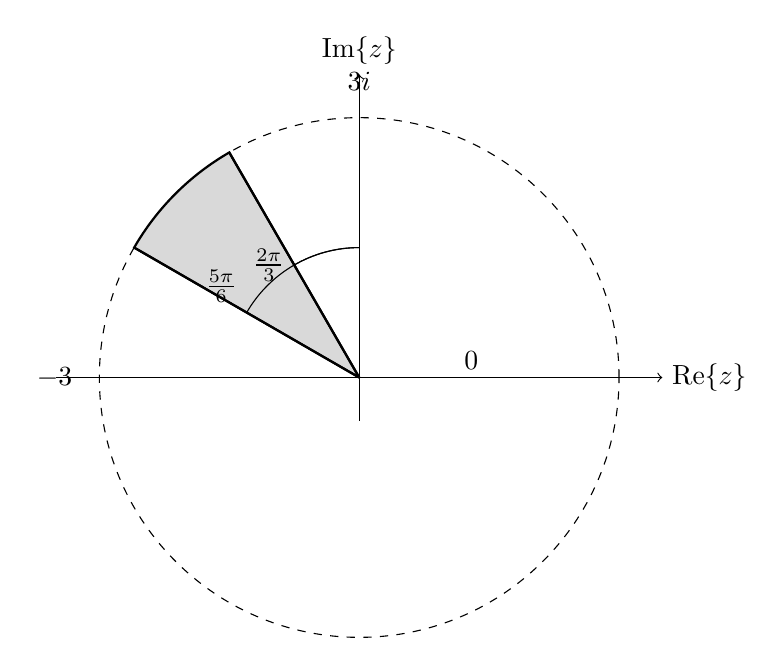
\begin{tikzpicture}[scale=1.1]
    % Ejes
    \draw[->] (-3.5,0) -- (3.5,0) node[right] {Re$\{z\}$};
    \draw[->] (0,-0.5) -- (0,3.5) node[above] {Im$\{z\}$};

    % Límites del sector
    \filldraw[fill=gray!30, draw=black, thick, domain=120:150, variable=\t]
        (0,0) -- ({3*cos(120)},{3*sin(120)})
        arc (120:150:3) -- (0,0);

    % Círculo de radio 3 (guía)
    \draw[dashed] (0,0) circle (3);

    % Radios
    \draw[thick] (0,0) -- ({3*cos(120)},{3*sin(120)});
    \draw[thick] (0,0) -- ({3*cos(150)},{3*sin(150)});

    % Etiquetas de ángulos
    \draw (1.1,0.2) node[right] {$0$};
    \draw (-3.2,0) node[left] {$-3$};
    \draw (0,3.2) node[above] {$3i$};
    \draw (0,1.5) arc (90:120:1.5) node[left] {$\frac{2\pi}{3}$};
    \draw (0,1.5) arc (90:150:1.5) node[above left] {$\frac{5\pi}{6}$};
\end{tikzpicture}
\caption{Representación de la región del problema \ref{comprepex}}
\end{figure}

Por lo tanto, el conjunto pedido es el sector sombreado en la figura, correspondiente a los números complejos con argumento entre $\frac{2\pi}{3}$ y $\frac{5\pi}{6}$ y módulo menor que $3$.
\end{myproof}

\end{prob}

\begin{prob}\label{compubicacion}
En el plano complejo se han dibujado los números complejos $z$ y $w$ como se muestra en la figura. Indique en la misma figura dónde quedarían aproximadamente los números: 


\begin{enumerate}[$a)$]
\item $\dfrac{1}{z}$
\item $(1+i)z$
\item $\overline{w}$ 
\item $-z$ 
\item $w^2$
\end{enumerate}		
		
\begin{figure}[H]
\centering
\begin{tikzpicture}[scale=1.5]
    % Ejes coordenados
    \draw[->] (-1.3,0) -- (1.5,0) node[above left] {Re};
    \draw[->] (0,-1.35) -- (0,1.75) node[below right] {Im};
    
    % Marcas en los ejes
    \draw (1,-2pt) -- (1,2pt) node[above] {$1$};
    \draw (-2pt,1) -- (2pt,1) node[right] {$i$};
    
    % Círculo unitario punteado
    \draw[dashed] (0,0) circle (1);
    
    % Vector z (primer cuadrante, 45°)
    \draw[->, thick] (0,0) -- (0.707,0.707);
    \node at (0.7,0.8) {$z$};
    
    % Vector w (segundo cuadrante)
    \draw[->, thick] (0,0) -- (-0.355,0.352);
    \node at (-0.5,0.5) {$w$};
    
\end{tikzpicture}
\caption{Figura del problema \ref{compubicacion}}
\end{figure}
\begin{myproof}
Analicemos la ubicación aproximada de cada número pedido, usando la información de la figura: $z$ está en el primer cuadrante, sobre la circunferencia unitaria, formando $45^\circ$ con el eje real, es decir, $z = \frac{\sqrt{2}}{2} + i\frac{\sqrt{2}}{2}$ mientras que $w$ está en el segundo cuadrante, también sobre la circunferencia unitaria, aproximadamente a $135^\circ$, es decir, $w \approx -\frac{\sqrt{2}}{2} + i\frac{\sqrt{2}}{2}$.

Ahora ubicamos cada número:

\begin{enumerate}[a)]
\item $\dfrac{1}{z}:$ Como $|z|=1$, $\frac{1}{z} = \overline{z}$, es decir, el conjugado de $z$. Así, $\frac{1}{z}$ estará en el primer cuadrante, sobre el círculo unitario, pero reflejado respecto al eje real aproximadamente en $(\frac{\sqrt{2}}{2}, -\frac{\sqrt{2}}{2})$.

\item $(1+i)z:$ Multiplicar por $1+i$ equivale a multiplicar el módulo por $\sqrt{2}$ y girar $45^\circ$. Como $z$ ya está a $45^\circ$, sumamos $45^\circ$ y obtenemos $90^\circ$ (es decir, sobre el eje imaginario positivo) y el módulo es $1 \cdot \sqrt{2} = \sqrt{2}$. Así, $(1+i)z$ estará en el eje $i$, a una distancia $\sqrt{2}$ del origen.

\item $\overline{w}:$ El conjugado de $w$ se obtiene reflejando $w$ respecto al eje real. Así, $\overline{w}$ estará en el cuarto cuadrante, en el punto $(-\frac{\sqrt{2}}{2}, -\frac{\sqrt{2}}{2})$.

\item $-z$ es el opuesto de $z$, es decir, el mismo módulo pero dirección opuesta: estará en el tercer cuadrante, en $(-\frac{\sqrt{2}}{2}, -\frac{\sqrt{2}}{2})$.

\item Como $w$ tiene módulo $1$ y argumento $135^\circ$ ($\frac{3\pi}{4}$), al elevar al cuadrado, el módulo sigue siendo $1$ y el argumento se duplica: $2 \cdot 135^\circ = 270^\circ$ ($\frac{3\pi}{2}$), que corresponde al eje imaginario negativo, es decir, en $-i$.
\end{enumerate}

A continuación se muestra la figura con las ubicaciones aproximadas:

\begin{figure}[H]
\centering
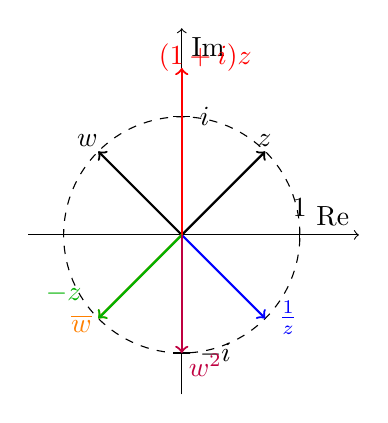
\begin{tikzpicture}[scale=1.5]
    % Ejes coordenados
    \draw[->] (-1.3,0) -- (1.5,0) node[above left] {Re};
    \draw[->] (0,-1.35) -- (0,1.75) node[below right] {Im};
    
    % Marcas en los ejes
    \draw (1,-2pt) -- (1,2pt) node[above] {$1$};
    \draw (-2pt,1) -- (2pt,1) node[right] {$i$};
    \draw (-2pt,-1) -- (2pt,-1) node[right] {$-i$};
    
    % Círculo unitario punteado
    \draw[dashed] (0,0) circle (1);
    
    % Vector z (primer cuadrante, 45°)
    \draw[->, thick] (0,0) -- (0.707,0.707);
    \node at (0.7,0.8) {$z$};
    
    % Vector w (segundo cuadrante)
    \draw[->, thick] (0,0) -- (-0.707,0.707);
    \node at (-0.8,0.8) {$w$};
    
    % (a) 1/z
    \draw[->, thick, blue] (0,0) -- (0.707,-0.707);
    \node[blue] at (0.9,-0.7) {$\frac{1}{z}$};
    
    % (b) (1+i)z
    \draw[->, thick, red] (0,0) -- (0,1.414);
    \node[red] at (0.2,1.5) {$(1+i)z$};
    
    % (c) conjugado de w
    \draw[->, thick, orange] (0,0) -- (-0.707,-0.707);
    \node[orange] at (-0.85,-0.75) {$\overline{w}$};
    
    % (d) -z
    \draw[->, thick, green!70!black] (0,0) -- (-0.707,-0.707);
    \node[green!70!black] at (-1.0,-0.5) {$-z$};
    
    % (e) w^2
    \draw[->, thick, purple] (0,0) -- (0,-1);
    \node[purple] at (0.2,-1.1) {$w^2$};
\end{tikzpicture}
\caption{Solución del problema \ref{compubicacion}}
\end{figure}

Así, cada número queda representado en la figura en su ubicación aproximada.
\end{myproof}

\end{prob}
	
\begin{prob} La ecuación $2z^4+2z^2+1=0$ tiene una raíz compleja $z$ con argumento entre $\pi$ y $\dfrac{3\pi}{2}$. Determine el argumento de $z$.
\begin{myproof}
Primero, reescribimos la ecuación \(2z^4 + 2z^2 + 1 = 0,\) dividiendo entre $2,$ \(
z^4 + z^2 + \frac{1}{2} = 0.\)


Hacemos el cambio $w = z^2:$ \(
w^2 + w + \frac{1}{2} = 0
\) y resolvemos la ecuación cuadrática:
\[
w = \frac{-1 \pm \sqrt{1 - 2}}{2} = \frac{-1 \pm i}{2}
\]

Ahora, buscamos $z$ tal que $z^2 = w$ y su argumento esté entre $\pi$ y $\frac{3\pi}{2}$.

Tomamos $w_1 = \frac{-1 + i}{2}$ y $w_2 = \frac{-1 - i}{2}$.

Calculamos el argumento de $w_1$: \(
\arg(w_1) = \arctan\left(\frac{1}{-1}\right) = \arctan(-1).\)


Como $w_1$ está en el segundo cuadrante, su argumento es: \(\pi - \frac{\pi}{4} = \frac{3\pi}{4} \) y su módulo es: \[|w_1| = \sqrt{\left(\frac{-1}{2}\right)^2 + \left(\frac{1}{2}\right)^2} = \frac{1}{\sqrt{2}}.\]

Las raíces cuadradas de $w_1$ son: \(
z = \left(\frac{1}{\sqrt{2}}\right)^{1/2} e^{\left(i \dfrac{\frac{3\pi}{4} + 2k\pi}{2}\right)}, \quad k=0,1
\)

Los argumentos posibles son: \(
\theta_1 = \frac{3\pi}{8}, \quad \theta_2 = \frac{3\pi}{8} + \pi = \frac{11\pi}{8}
\)

Ahora, como $\frac{11\pi}{8}$ está entre $\pi$ y $\frac{3\pi}{2},$  el argumento de la raíz $z$ pedida es: \(
\boxed{\frac{11\pi}{8}}
\)
\end{myproof}

\end{prob}		

\begin{prob}Use la fórmula de De Moivre para encontrar todas las raíces complejas del polinomio $z^6-11(i+1)z^3+121i=0$.
\begin{myproof}
Dada la ecuación \(
z^6 - 11(1+i)z^3 + 121i = 0
\) hacemos el cambio $w = z^3$, así que la ecuación se convierte en:
\[
w^2 - 11(1+i)w + 121i = 0
\]
Usando factor común por agrupación: \begin{align*}
w^2 - 11(1+i)w + 121i &= 0 \\
w^2 - 11w - 11iw + 121i &= 0 \\
(w^2 - 11w) - (11iw - 121i) &= 0 \\
w(w - 11) -11i(w - 11) &= 0 \\
(w - 11)(w - 11i) &= 0
\end{align*}

Por lo tanto, las raíces para $w$ son: \(
w_1 = 11 \) y \(w_2 = 11i.\) Ahora resolvemos $z^3 = w$ para cada $w$:

\textbf{Para $w_1 = 11$:}
\[
z^3 = 11 \implies z = 11^{1/3} \cdot e^{i\dfrac{2\pi k}{3}}, \quad k=0,1,2
\]
Esto da las tres raíces:
\[
z_1 = 11^{1/3}
\]
\[
z_2 = 11^{1/3} \cdot e^{i\dfrac{2\pi}{3}} = 11^{1/3} \left(-\frac{1}{2} + i\frac{\sqrt{3}}{2}\right)
\]
\[
z_3 = 11^{1/3} \cdot e^{i\dfrac{4\pi}{3}} = 11^{1/3} \left(-\frac{1}{2} - i\frac{\sqrt{3}}{2}\right)
\]

\textbf{Para $w_2 = 11i$:}
\[
w_2 = 11i = 11 e^{i\frac{\pi}{2}}
\]
Entonces,
\[
z^3 = 11i \implies z = 11^{1/3} e^{i\dfrac{\frac{\pi}{2} + 2\pi k}{3}}, \quad k=0,1,2
\]
Esto da las tres raíces:
\[
z_4 = 11^{1/3} e^{i\dfrac{\pi}{6}} = 11^{1/3} \left(\frac{\sqrt{3}}{2} + i\frac{1}{2}\right)
\]
\[
z_5 = 11^{1/3} e^{i\dfrac{5\pi}{6}} = 11^{1/3} \left(-\frac{\sqrt{3}}{2} + i\frac{1}{2}\right)
\]
\[
z_6 = 11^{1/3} e^{i\frac{3\pi}{2}} = 11^{1/3} (-i)
\]

\textbf{En resumen, las seis raíces complejas son:}
\[
\boxed{
\begin{aligned}
z_1 &= 11^{1/3} \\\\
z_2 &= 11^{1/3} \left(-\frac{1}{2} + i\frac{\sqrt{3}}{2}\right) \\\\
z_3 &= 11^{1/3} \left(-\frac{1}{2} - i\frac{\sqrt{3}}{2}\right) \\\\
z_4 &= 11^{1/3} \left(\frac{\sqrt{3}}{2} + i\frac{1}{2}\right) \\\\
z_5 &= 11^{1/3} \left(-\frac{\sqrt{3}}{2} + i\frac{1}{2}\right) \\\\
z_6 &= 11^{1/3} (-i)
\end{aligned}
}
\]
Todas las raíces se obtuvieron usando la fórmula de De Moivre.
\end{myproof}
\end{prob}

\begin{prob} 
Determine el valor de verdad de las siguientes afirmaciones donde $z, w \in \mathbb{C}$. Si son verdaderas demuéstrelas; si son falsas, muestre un contraejemplo.

\begin{enumerate}[$a)$]
\item  $|z|=|iz|$
\item  Si $z$ y $w$ son imaginarios puros, entonces $zw$ es imaginario puro.
\item  Si $z\neq \mathbf{0}$, entonces $\left|\dfrac{z}{|z|}\right|=1$
\item  Si $re^{i\theta}$ es la forma polar de $z$, entonces $\text{Im}(z)=r\sin \theta$
\item $\arg(z)=-\arg(\overline{z})$
\item  Si $z$ y $\overline{z}$ son raíces de $ax^2+bx+c=0$, entonces $b^2-4ac<0$
\item  Sean $z, w\in \mathbb{C}$. Si $|w|<1$ y $|z|\leq 1$, entonces $\left|\dfrac{z+w}{1+\overline{w}z}\right|=1$
\item  Si $z$ y $w$ son imaginarios puros, entonces $zw\in \mathbb{R}$
\item  $z=\overline{z}$ si y solo si $z$ es real
\item  Si $z$ es imaginario puro, entonces $z^{-1}=-z$
\item  Si $\overline{z}=-z$, entonces $z$ es imaginario puro
\item  Si $z=a+bi$ con $a=b$, entonces $|z|=|a|\sqrt{2}$
\item  Si $z=bi$ con $b\neq 0$, entonces $iz$ es real
\end{enumerate}
\begin{myproof}
Analizamos cada afirmación:

\begin{enumerate}[a)]
\item \textbf{$|z|=|iz|$}

Verdadera.  
Demostración: Si $z = a + bi$, entonces $iz = i(a+bi) = -b + ai$.  
\[
|iz| = \sqrt{(-b)^2 + a^2} = \sqrt{a^2 + b^2} = |z|
\]

\item \textbf{Si $z$ y $w$ son imaginarios puros, entonces $zw$ es imaginario puro.}

Falsa.  
Contraejemplo: Sea $z = 2i$, $w = 3i$. Entonces $zw = (2i)(3i) = 6i^2 = -6$, que es real, no imaginario puro.

\item \textbf{Si $z\neq \mathbf{0}$, entonces $\left|\dfrac{z}{|z|}\right|=1$}

Verdadera.  
Demostración:  
\[
\left|\frac{z}{|z|}\right| = \frac{|z|}{|z|} = 1
\]

\item \textbf{Si $re^{i\theta}$ es la forma polar de $z$, entonces $\text{Im}(z)=r\sin \theta$}

Verdadera.  
Demostración:  
\[
z = re^{i\theta} = r(\cos\theta + i\sin\theta) \implies \text{Im}(z) = r\sin\theta
\]

\item \textbf{$\arg(z)=-\arg(\overline{z})$}

Verdadera.  
Demostración: Si $z = re^{i\theta}$, entonces $\overline{z} = re^{-i\theta}$, así que $\arg(\overline{z}) = -\theta$, por lo tanto $\arg(z) = -\arg(\overline{z})$.

\item \textbf{Si $z$ y $\overline{z}$ son raíces de $ax^2+bx+c=0$, entonces $b^2-4ac<0$}

Verdadera.  
Demostración: Si las raíces son conjugadas, el discriminante es negativo, pues sólo ocurre si no hay raíces reales.

\item \textbf{Sean $z, w\in \mathbb{C}$. Si $|w|<1$ y $|z|\leq 1$, entonces $\left|\dfrac{z+w}{1+\overline{w}z}\right|=1$}

Falsa.  
Contraejemplo: Sea $z=0$, $w=0.5$. Entonces
\[
\left|\frac{0+0.5}{1+0}\right| = 0.5 \neq 1
\]

\item \textbf{Si $z$ y $w$ son imaginarios puros, entonces $zw\in \mathbb{R}$}

Verdadera.  
Demostración: $z=ai$, $w=bi$ con $a,b\in\mathbb{R}$. Entonces $zw = (ai)(bi) = ab(i^2) = ab(-1) \in \mathbb{R}$.

\item \textbf{$z=\overline{z}$ si y sólo si $z$ es real}

Verdadera.  
Demostración: $z=a+bi$, $\overline{z}=a-bi$. $z=\overline{z}$ implica $b=0$.

\item \textbf{Si $z$ es imaginario puro, entonces $z^{-1}=-z$}

Falsa.  
Contraejemplo: Sea $z=2i$. Entonces $z^{-1} = \frac{1}{2i} = -\frac{i}{2} \neq -2i$.

\item \textbf{Si $\overline{z}=-z$, entonces $z$ es imaginario puro}

Verdadera.  
Demostración: $z=a+bi$, $\overline{z}=a-bi$. Si $\overline{z}=-z$, entonces $a-bi = -a-bi \implies a=0$, así que $z=bi$.

\item \textbf{Si $z=a+bi$ con $a=b$, entonces $|z|=|a|\sqrt{2}$}

Verdadera.  
Demostración: $|z| = \sqrt{a^2 + a^2} = |a|\sqrt{2}$.

\item \textbf{Si $z=bi$ con $b\neq 0$, entonces $iz$ es real}

Verdadera.  
Demostración: $iz = i(bi) = b(i^2) = b(-1) = -b \in \mathbb{R}$.
\end{enumerate}
\end{myproof}

\end{prob}

\begin{prob} (\cite{andreescu2014complex}, p. 19, Problema 9) Encuentre los números reales $x, y$ en cada caso:
\begin{enumerate}[$a)$]
\item $(1-2i)x + (1+2i)y=1+i$
\item $(4-3i)x^2+(3+2i)xy=4y^2-\dfrac{1}{2}x^2+(3xy-2y^2)i$
\end{enumerate}
\begin{myproof}
Resolvamos cada inciso por separado.

\textbf{a)} \quad $(1-2i)x + (1+2i)y = 1 + i$

Expresamos la ecuación en términos de partes reales e imaginarias:
\[
[(1)x + (1)y] + [-2x + 2y]i = 1 + i
\]
\[
(x + y) + (-2x + 2y)i = 1 + i
\]
Igualando partes reales e imaginarias:
\[
\begin{cases}
x + y = 1 \\
-2x + 2y = 1
\end{cases}
\]
Resolviendo el sistema:
\[
x + y = 1 \implies x = 1 - y
\]
\[
-2(1 - y) + 2y = 1 \implies -2 + 2y + 2y = 1 \implies 4y = 3 \implies y = \frac{3}{4}
\]
\[
x = 1 - \frac{3}{4} = \frac{1}{4}
\]

\textbf{Solución:} $\boxed{x = \frac{1}{4},\quad y = \frac{3}{4}}$

\vspace{1em}

\textbf{b)} \quad $(4-3i)x^2 + (3+2i)xy = 4y^2 - \dfrac{1}{2}x^2 + (3xy - 2y^2)i$

Llevamos todos los términos al mismo lado e igualamos partes reales e imaginarias:
\[
(4-3i)x^2 + (3+2i)xy - 4y^2 + \frac{1}{2}x^2 - (3xy-2y^2)i = 0
\]
\[
\bigg[4x^2 + \frac{1}{2}x^2 + 3xy - 4y^2\bigg] + \bigg[-3x^2 + 2xy - (3xy - 2y^2)\bigg]i = 0
\]
\[
\left(\frac{9}{2}x^2 + 3xy - 4y^2\right) + \left(-3x^2 + 2xy - 3xy + 2y^2\right)i = 0
\]
\[
\left(\frac{9}{2}x^2 + 3xy - 4y^2\right) + \left(-3x^2 - xy + 2y^2\right)i = 0
\]
Igualamos a cero cada parte:
\[
\begin{cases}
\frac{9}{2}x^2 + 3xy - 4y^2 = 0 \\
-3x^2 - xy + 2y^2 = 0
\end{cases}
\]

Resolvemos el sistema. La segunda ecuación:
\[
-3x^2 - xy + 2y^2 = 0 \implies 3x^2 + xy - 2y^2 = 0
\]
\[
x(3x + y) = 2y^2
\]
Si $y = 0$, entonces $x = 0$ (única solución trivial).

Si $y \neq 0$, despejamos $x$ en términos de $y$:
\[
3x^2 + xy - 2y^2 = 0
\]
\[
x = \frac{-y \pm \sqrt{y^2 + 24y^2}}{6} = \frac{-y \pm 5y}{6}
\]
\[
x_1 = \frac{4y}{6} = \frac{2y}{3}, \quad x_2 = \frac{-6y}{6} = -y
\]
Probamos $x = \frac{2y}{3}$ en la primera ecuación:
\[
\frac{9}{2}\left(\frac{4y^2}{9}\right) + 3\left(\frac{2y}{3}\right)y - 4y^2 = 2y^2 + 2y^2 - 4y^2 = 0
\]
Por lo tanto, $x = \frac{2y}{3}$, $y$ arbitrario.

\textbf{Soluciones:}
\[
\boxed{
\begin{aligned}
&x = 0,\quad y = 0 \\
&x = \frac{2}{3}y,\quad y\in\mathbb{R}
\end{aligned}
}
\]
\end{myproof}
\end{prob}

\begin{prob} (\cite{andreescu2014complex}, p. 21, Problema 31) Sean $z_1, z_2, z_3$ números complejos tales que $z_1+z_2+z_3=0$ y $|z_1|=|z_2|=|z_3|=1$. Demuestre que $z_1^2+z_2^2+z_3^2=0$.
\begin{myproof}
Sean $z_1, z_2, z_3 \in \mathbb{C}$ tales que $z_1 + z_2 + z_3 = 0$ y $|z_1| = |z_2| = |z_3| = 1$.

Queremos demostrar que $z_1^2 + z_2^2 + z_3^2 = 0$.

Como $z_1 + z_2 + z_3 = 0$, tenemos $z_3 = -z_1 - z_2$. Sustituimos en la suma de los cuadrados:
\[
z_1^2 + z_2^2 + z_3^2 = z_1^2 + z_2^2 + (-z_1 - z_2)^2
\]
\[
= z_1^2 + z_2^2 + (z_1^2 + 2z_1z_2 + z_2^2)
\]
\[
= z_1^2 + z_2^2 + z_1^2 + 2z_1z_2 + z_2^2
\]
\[
= 2z_1^2 + 2z_2^2 + 2z_1z_2
\]
\[
= 2(z_1^2 + z_2^2 + z_1z_2)
\]

Por otro lado, usando la condición de los módulos, notamos que $z_1, z_2, z_3$ son puntos en la circunferencia unitaria y suman cero; es decir, forman un triángulo equilátero centrado en el origen. Así, existen $\theta \in \mathbb{R}$ tal que:
\[
z_1 = e^{i\theta},\quad z_2 = e^{i(\theta + 2\pi/3)},\quad z_3 = e^{i(\theta + 4\pi/3)}
\]
Calculamos la suma de los cuadrados:
\[
z_1^2 + z_2^2 + z_3^2 = e^{i2\theta} + e^{i[2(\theta + 2\pi/3)]} + e^{i[2(\theta + 4\pi/3)]}
\]
\[
= e^{i2\theta} + e^{i(2\theta + 4\pi/3)} + e^{i(2\theta + 8\pi/3)}
\]
Pero $8\pi/3 = 2\pi + 2\pi/3$, así que $e^{i(2\theta + 8\pi/3)} = e^{i(2\theta + 2\pi/3)}$.

Entonces,
\[
z_1^2 + z_2^2 + z_3^2 = e^{i2\theta} + e^{i(2\theta + 4\pi/3)} + e^{i(2\theta + 2\pi/3)}
\]
\[
= e^{i2\theta} + e^{i(2\theta + 2\pi/3)} + e^{i(2\theta + 4\pi/3)}
\]
Esta suma es la suma de las raíces cúbicas de la unidad multiplicadas por $e^{i2\theta}$:
\[
e^{i2\theta} \left[1 + e^{i2\pi/3} + e^{i4\pi/3}\right]
\]
Pero $1 + e^{i2\pi/3} + e^{i4\pi/3} = 0$.

Por lo tanto,
\[
z_1^2 + z_2^2 + z_3^2 = 0
\]
\end{myproof}
\end{prob}

\begin{prob} 
Encuentre la forma polar de los siguientes números complejos. ¿Cuál es el efecto geométrico de multiplicar y dividir por cada uno? Justifique su respuesta.
\begin{multicols}{3}
\begin{enumerate}[$a)$]
\item $z=3+i$
\item $z=5-i$
\item $z=8$
\end{enumerate}
\end{multicols}
\begin{myproof} Multiplicar por un número complejo $re^{i\theta}$ equivale a: Multiplicar el módulo por $r$ (dilatar o contraer la distancia al origen) y sumar $\theta$ al argumento (girar en sentido antihorario). Por otro lado, dividir equivale a dividir el módulo entre $r$ y restar $\theta$ al argumento (girar en sentido horario). Analicemos cada número complejo:

\textbf{a) $z = 3 + i:$} El módulo es $r = \sqrt{3^2 + 1^2} = \sqrt{10}$ y su argumento es $\theta = \arctan\left(\frac{1}{3}\right)$.  Así, la forma polar es \(
  z = \sqrt{10} \, e^{i\arctan(1/3)}. \) El efecto geométrico de multiplicar por $z$ será multiplicar el módulo por $\sqrt{10}$ y girar el ángulo $\arctan(1/3)$ en sentido antihorario, mientras que dividir por $z$ implica dividir el módulo entre $\sqrt{10}$ y gira el ángulo $-\arctan(1/3)$ en sentido horario.

\textbf{b) $z = 5 - i:$} El módulo es $r = \sqrt{5^2 + (-1)^2} = \sqrt{26}$ y su  argumento es $\theta = \arctan\left(\frac{-1}{5}\right)$. Así, la forma polar es \(
  z = \sqrt{26} \, e^{i\arctan(-1/5)}.\) El efecto geométrico de multiplicar por $z$ será multiplicar el módulo por $\sqrt{26}$ y girar el ángulo $\arctan(-1/5)$ en sentido antihorario mientras que dividir por $z$ divide el módulo entre $\sqrt{26}$ y gira el ángulo $-\arctan(-1/5)$ en sentido horario.

\textbf{c) $z = 8:$} El módulo es $r = 8$ y el argumento es $\theta = 0$. Así, la forma polar es \(z = 8\, e^{i\cdot 0} = 8.\) El efecto geométrico de multiplicar por $z$ será multiplicar el módulo por $8$ y no gira el ángulo (no hay rotación) mientras que para dividir por $z$ se divide el módulo entre $8$ y no hay rotación.

\end{myproof}

\end{prob}

\begin{prob} (\cite{andreescu2014complex}, p. 55, Problema 5) Use la fórmula de De Moivre para encontrar las raíces cuartas de:
\begin{multicols}{2}
\begin{enumerate}[$a)$]
\item $z=-27$
\item $z=-7+24i$
\end{enumerate}
\end{multicols}
\begin{myproof}
Vamos a encontrar las raíces cuartas de cada número complejo usando la fórmula de De Moivre.

\textbf{a) $z = -27:$} El módulo es $r = 27$ y el argumento es $\theta = \pi$ (pues $-27$ está sobre el eje real negativo). Las raíces cuartas de $z$ son:
\[
w_k = 27^{1/4} \cdot e^{i\dfrac{\pi + 2\pi k}{4}}, \quad k = 0,1,2,3
\]

Por lo tanto, las raíces cuartas son:
\[
\boxed{
\begin{aligned}
w_0 &= 27^{1/4} \, e^{i\frac{\pi}{4}} = 27^{1/4} \left(\frac{\sqrt{2}}{2} + i\frac{\sqrt{2}}{2}\right) \\
w_1 &= 27^{1/4} \, e^{i\frac{3\pi}{4}} = 27^{1/4} \left(-\frac{\sqrt{2}}{2} + i\frac{\sqrt{2}}{2}\right) \\
w_2 &= 27^{1/4} \, e^{i\frac{5\pi}{4}} = 27^{1/4} \left(-\frac{\sqrt{2}}{2} - i\frac{\sqrt{2}}{2}\right) \\
w_3 &= 27^{1/4} \, e^{i\frac{7\pi}{4}} = 27^{1/4} \left(\frac{\sqrt{2}}{2} - i\frac{\sqrt{2}}{2}\right)
\end{aligned}
}
\]

\textbf{b) $z = -7 + 24i:$} El módulo: $r = \sqrt{(-7)^2 + 24^2} = \sqrt{49 + 576} = \sqrt{625} = 25.$  Como $-7 < 0$ y $24 > 0$, el número está en el segundo cuadrante. El argumento es \(
\theta = \pi - \arctan\left(\frac{24}{7}\right)
\)

Las raíces cuartas de $z$ son:
\[
\boxed{
w_k = \sqrt{5} \cdot e^{i\left(\frac{\pi - \arctan\left(\frac{24}{7}\right)}{4} + \frac{\pi k}{2}\right)}, \quad k = 0,1,2,3
}
\]
para $k = 0,1,2,3$.

\end{myproof}

\end{prob}

\begin{prob}  (\cite{andreescu2014complex}, p. 55, Problema 7) Use la fórmula de De Moivre para encontrar todas las raíces complejas de:
\begin{multicols}{2}
\begin{enumerate}[$a)$]
\item $z^4+16=0$
\item $z^3-27i=0$
\item $z^5-1-i=0$
\item $(2-3i)z^6+1+5i=0$
\end{enumerate}
\end{multicols}
\begin{myproof}
Resolvamos cada inciso usando la fórmula de De Moivre.

\textbf{a)} $z^4 + 16 = 0\Rightarrow z^4 = -16 = 16 e^{i\pi}$

Las raíces cuartas son: \(
z_k = 16^{1/4} e^{i \dfrac{\pi + 2\pi k}{4}}, \quad k = 0,1,2,3
\)

Explícitamente:
\[
\boxed{
\begin{aligned}
z_0 &= 2 e^{i\frac{\pi}{4}} = \sqrt{2} + i\sqrt{2} \\
z_1 &= 2 e^{i\frac{3\pi}{4}} = -\sqrt{2} + i\sqrt{2} \\
z_2 &= 2 e^{i\frac{5\pi}{4}} = -\sqrt{2} - i\sqrt{2} \\
z_3 &= 2 e^{i\frac{7\pi}{4}} = \sqrt{2} - i\sqrt{2}
\end{aligned}
}
\]

\vspace{1em}

\textbf{b)} $z^3 - 27i = 0 \Rightarrow z^3 = 27i = 27 e^{i\frac{\pi}{2}}.$
Las raíces cúbicas son \( z_k = 27^{1/3} e^{i \dfrac{\frac{\pi}{2} + 2\pi k}{3}}, \quad k=0,1,2.
\)
Explícitamente: 
\[
\boxed{
\begin{aligned}
z_0 &= 3 e^{i\frac{\pi}{6}} = \frac{3\sqrt{3}}{2} + i\frac{3}{2} \\
z_1 &= 3 e^{i\frac{5\pi}{6}} = -\frac{3\sqrt{3}}{2} + i\frac{3}{2} \\
z_2 &= 3 e^{i\frac{3\pi}{2}} = -3i
\end{aligned}
}
\]


\textbf{c)} $z^5 - 1 - i = 0\Rightarrow z^5 = 1 + i = \sqrt{2} e^{i\frac{\pi}{4}}.$ Las raíces quintas son 
\[
\boxed{
z_k = 2^{1/10} \, e^{i\left( \dfrac{\pi}{20} + \dfrac{2\pi k}{5} \right ) }, \quad k=0,1,2,3,4
}
\]


\textbf{d)} $(2-3i)z^6 + 1 + 5i = 0\Rightarrow (2-3i)z^6 = -1 - 5i\Rightarrow z^6 = \frac{-1 - 5i}{2 - 3i}.$


Multiplicamos numerador y denominador por el conjugado del denominador:
\[
\frac{-1 - 5i}{2 - 3i} \cdot \frac{2 + 3i}{2 + 3i} = \frac{(-1 - 5i)(2 + 3i)}{(2)^2 + (3)^2}
\]
Calculamos el numerador:
\[
(-1 - 5i)(2 + 3i) = -2 - 3i - 10i - 15i^2 = -2 - 13i + 15 = 13 - 13i
\]
El denominador es $4 + 9 = 13$.

\[
z^6 = \frac{13 - 13i}{13} = 1 - i = \sqrt{2} e^{-i\frac{\pi}{4}}
\]
Las raíces sextas son:
\[
\boxed{
z_k = 2^{1/12} \, e^{i\left( -\frac{\pi}{24} + \frac{\pi k}{3} \right ) }, \quad k=0,1,2,3,4,5
}
\]

\end{myproof}

\end{prob}

\begin{prob} 
Demuestre que $z$ es imaginario puro si y solo si $z=-\overline{z}$.
\begin{myproof}
Sea $z \in \mathbb{C}$. Recordemos que $z$ es imaginario puro si y solo si su parte real es cero, es decir, $z = bi$ con $b \in \mathbb{R}$.

\textbf{($\Rightarrow$)} Supongamos que $z$ es imaginario puro.  
Entonces $z = bi$ con $b \in \mathbb{R}$.  
El conjugado es $\overline{z} = \overline{bi} = -bi$.  
Por lo tanto,
\[
-\overline{z} = -(-bi) = bi = z.
\]
Así, $z = -\overline{z}$.

\textbf{($\Leftarrow$)} Supongamos que $z = -\overline{z}$.  
Sea $z = a + bi$ con $a, b \in \mathbb{R}$.  
Entonces $\overline{z} = a - bi$ y la igualdad se convierte en:
\[
a + bi = - (a - bi) = -a + bi
\]
Comparando partes reales:
\[
a = -a \implies a = 0
\]
Por lo tanto, $z = 0 + bi = bi$, es decir, $z$ es imaginario puro.

\textbf{Conclusión:}  
$z$ es imaginario puro si y solo si $z = -\overline{z}$.
\end{myproof}

\end{prob}